\chapter{Biologie du cancer}\label{ch:b3:cancer-biology}

Une \omterm{def:b3:cancer-biology:hallmarks}{tumeur} assez grosse pour être palpée, d'un centimètre, contient un
milliard de cellules et résulte d'une trentaine de doublements à partir
d'une cellule qui a mal tourné --- typiquement une décennie de
croissance avant que quiconque l'ait su. Derrière cette cellule se
tiennent plusieurs mutations, dont chacune a dû survenir dans la même
lignée et dont chacune a supprimé l'un des contrôles des deux chapitres
précédents~: un frein à la division, un déclencheur de mort, une limite
au nombre de divisions, l'obligation de rester en place. Le \omterm{def:b3:cancer-biology:hallmarks}{cancer} est
l'évolution d'une population cellulaire à l'intérieur d'un corps, par
mutation et sélection, vers un état qui sert les cellules et tue
l'organisme. Ce chapitre traite des gènes qui sont touchés et de ce
qu'ils font normalement, de la statistique qui révèle combien de coups
sont nécessaires, de la physiologie qu'une \omterm{def:b3:cancer-biology:hallmarks}{tumeur} doit acquérir pour
dépasser le millimètre et pour se disséminer, des causes qu'on peut
éviter, et des traitements --- des poisons qui tuent les cellules en
division aux anticorps qui libèrent le système immunitaire --- que la
biologie a rendus possibles, ainsi que de la raison évolutive de leurs
échecs si fréquents.

\section{Ce qu'est un cancer}

\begin{definition}[Tumeur, cancer, caractères distinctifs]\label{def:b3:cancer-biology:hallmarks}
\index{cancer}\index{tumeur}\index{malin}\index{métastase}\index{caractères distinctifs du cancer}
Une \emph{tumeur} (néoplasme) est un clone de cellules qui a échappé
aux contrôles de sa croissance et s'accumule dans un tissu. Elle est
\emph{bénigne} si elle reste confinée et encapsulée, \emph{maligne} ---
un \emph{cancer} --- si ses cellules envahissent le tissu voisin et
sèment ailleurs des tumeurs secondaires (une \emph{métastase}), ce qui
est ce qui tue. Les cancers sont nommés d'après leur cellule
d'origine~: les carcinomes viennent des épithéliums (\qty{85}{\%} des
cancers humains), les sarcomes du tissu conjonctif, les leucémies et
les lymphomes des cellules hématopoïétiques, les gliomes de la glie.
Quel que soit le tissu, un clone malin a acquis le même jeu de
capacités, les \emph{caractères distinctifs du cancer}~: il prolifère
sans signaux de croissance extérieurs et ignore les signaux qui
devraient l'arrêter~; il résiste à l'\omterm{def:b3:cell-cycle-apoptosis:apoptosis}{apoptose}~; il se divise sans
limite, ayant réactivé la \omterm{def:b3:cancer-biology:telomerase}{télomérase}~; il induit des vaisseaux
sanguins~; il envahit et métastase~; et, sous tout cela, son génome est
instable, il reprogramme son métabolisme vers la glycolyse même en
présence de dioxygène (l'effet Warburg), il recrute des cellules
inflammatoires qui l'aident, et il échappe au système immunitaire.
Chaque caractère est un contrôle du tissu normal mis en échec, et
chacun se rapporte à des gènes.
\end{definition}

\begin{omfigure}
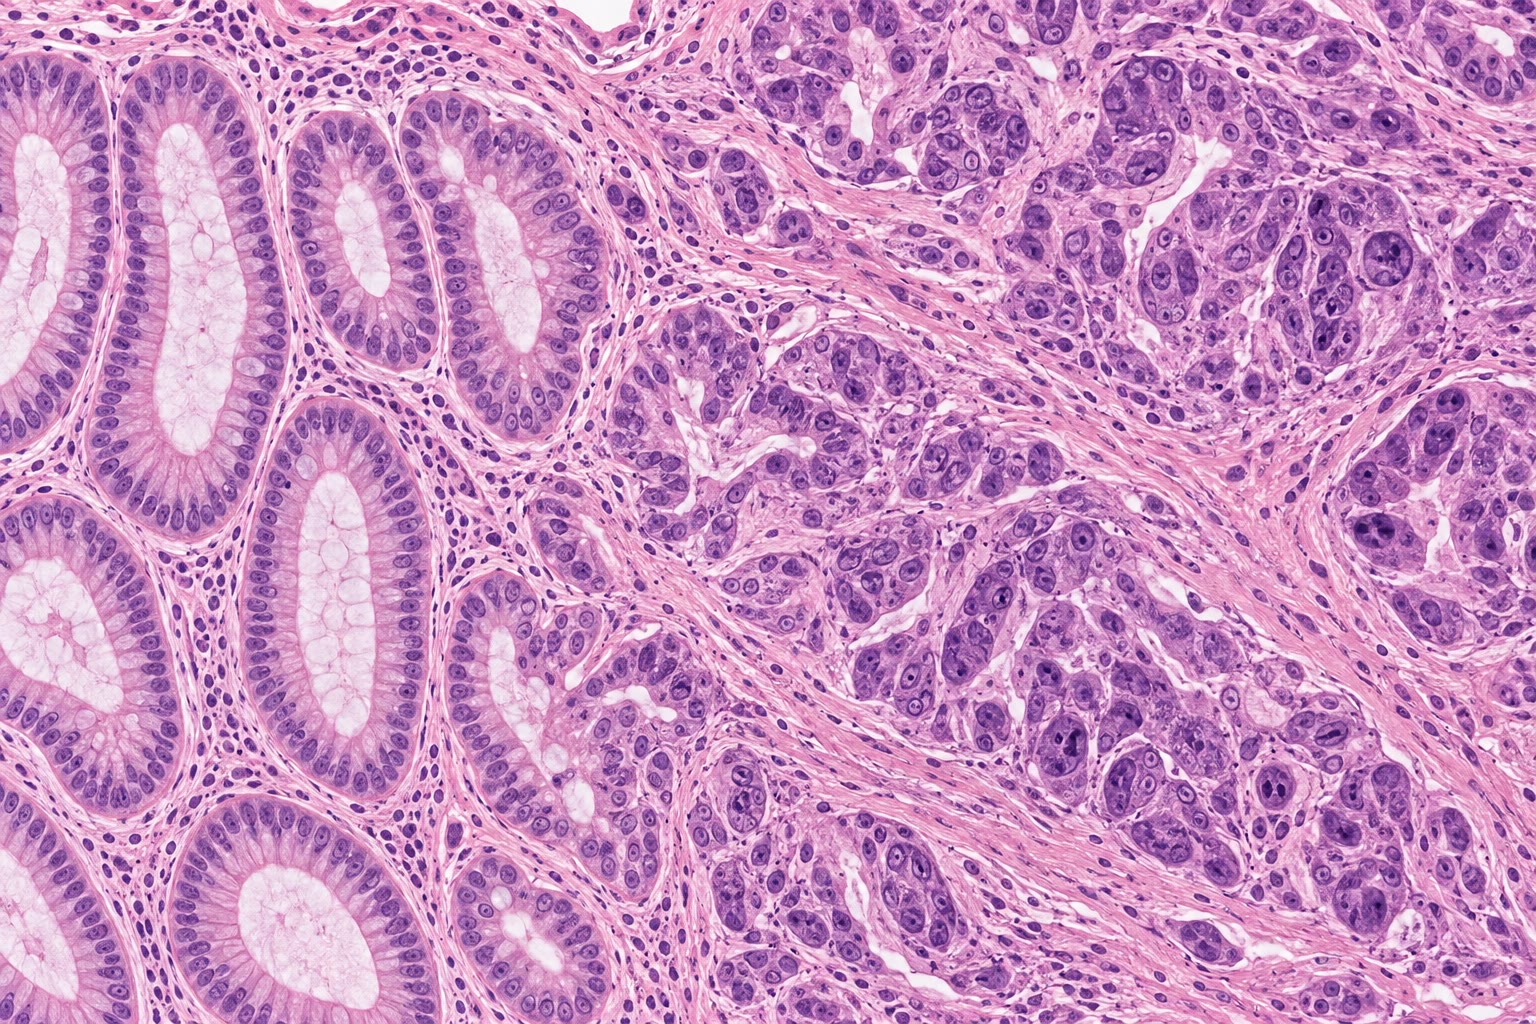
\includegraphics[width=0.56\linewidth]{images/book5/ai/b5-11-tumour-histology.jpg}

{\small Un carcinome à sa frontière~: à gauche, un épithélium
glandulaire ordonné aux noyaux réguliers~; à droite, des cellules
entassées aux noyaux gros et irréguliers qui envahissent le stroma
sous-jacent --- l'image que lit un anatomopathologiste pour déclarer
une \omterm{def:b3:cancer-biology:hallmarks}{tumeur} maligne.}
\end{omfigure}

\section{Les gènes qui sont touchés}

\begin{definition}[Oncogènes et gènes suppresseurs de tumeur]\label{def:b3:cancer-biology:genes}
\index{oncogène}\index{proto-oncogène}\index{gène suppresseur de tumeur}\index{Ras}\index{p53}\index{hypothèse des deux coups}
Un \emph{proto-oncogène} est un gène normal qui favorise la
prolifération ou la survie --- un facteur de croissance, son récepteur,
une protéine de signalisation, un facteur de transcription, une \omterm{def:b3:cell-cycle-apoptosis:cdk}{cycline}
--- et un \emph{oncogène} en est une forme mutante active sans son
signal normal~: une mutation ponctuelle qui bloque la \omterm{def:b3:membrane-traffic:coats}{petite GTPase}
\emph{Ras} sous sa forme GTP (la glycine~12 dans un quart de tous les
\omterm{def:b3:cancer-biology:hallmarks}{cancers}), une amplification du gène du récepteur HER2 ou du facteur de
transcription Myc, une translocation qui fusionne \emph{BCR} à la
kinase \emph{ABL} dans la leucémie myéloïde chronique ou place
\emph{MYC} à côté d'un amplificateur d'anticorps dans le lymphome de
Burkitt. Un seul allèle mutant suffit~: les oncogènes agissent de façon
dominante. Un \emph{gène suppresseur de \omterm{def:b3:cancer-biology:hallmarks}{tumeur}} freine la prolifération
ou impose la mort ou la réparation --- Rb et p16 au \omterm{def:b3:cell-cycle-apoptosis:checkpoints}{point de
restriction}, \emph{p53}, le gardien qui arrête ou tue une cellule
lésée, APC dans la \omterm{prop:b3:cancer-biology:pathways}{voie Wnt} du côlon, PTEN, BRCA1 et BRCA2, les gènes
de la \omterm{prop:b3:dna-repair:fidelity}{réparation des mésappariements} --- et il doit perdre ses deux
allèles pour contribuer~: \emph{deux coups}, le premier souvent hérité
dans les syndromes de \omterm{def:b3:cancer-biology:hallmarks}{cancer} familial, le second somatique. \emph{p53}
est muté dans la moitié de tous les \omterm{def:b3:cancer-biology:hallmarks}{cancers} humains et sa voie est
désactivée dans la plupart des autres.
\end{definition}

\begin{proof}[Faits expérimentaux]
Rous (1911) a transmis un sarcome de poule par un filtrat acellulaire,
un virus, dont l'unique gène transformant, \emph{src}, s'est révélé
chez Varmus et Bishop (1976) être une copie captée d'un gène normal de
poule --- les \omterm{def:b3:cancer-biology:genes}{oncogènes} sont des gènes cellulaires altérés. Weinberg
(1982) a transféré l'ADN d'un carcinome de vessie humain dans des
cellules de souris en culture, qui ont été transformées~; le fragment
responsable était \emph{RAS} avec un seul changement de base, et ce
changement était absent du tissu normal du patient. Knudson (1971) a
comparé des enfants atteints de la \omterm{def:b3:cancer-biology:hallmarks}{tumeur} oculaire qu'est le
rétinoblastome~: ceux qui avaient des antécédents familiaux
développaient plusieurs \omterm{def:b3:cancer-biology:hallmarks}{tumeurs} aux deux yeux, et tôt~; les autres une
seule, plus tard --- ce qui s'accorde avec des cas familiaux exigeant
un événement somatique, les cas sporadiques deux, et donc avec un gène
dont les deux copies doivent être perdues. \emph{RB} a été cloné en
1986 et ses deux allèles étaient bien inactivés dans chaque \omterm{def:b3:cancer-biology:hallmarks}{tumeur}.
\end{proof}

\begin{theorem}[Les coups et la courbe d'âge]\label{thm:b3:cancer-biology:armitage-doll}
\index{modèle d'Armitage--Doll}\index{cancérogenèse multi-étapes}
Supposons qu'un \omterm{def:b3:cancer-biology:hallmarks}{cancer} exige $k$ événements indépendants et limitants
dans une même lignée cellulaire, survenant chacun à la vitesse
constante $u$ par cellule et par an, dans une population de $N$
cellules sensibles, avec $ut \ll 1$. La probabilité qu'une cellule
donnée ait subi les $k$ événements à l'âge $t$ vaut alors environ
$(ut)^{k}$, le risque cumulé dans le tissu environ $N(ut)^{k}$, et
l'incidence --- les cas nouveaux par an à l'âge $t$ --- vaut
\[
I(t) \approx N\,k\,u^{k}\,t^{\,k-1},
\]
une puissance de l'âge d'exposant $k - 1$~: une droite de pente
$k - 1$ en échelle log--log. Pour une personne qui hérite l'un des
événements, le même \omterm{def:b3:cancer-biology:hallmarks}{cancer} a une incidence $\propto t^{\,k-2}$, une
puissance de moins.
\end{theorem}
\begin{proof}
Chaque événement, de vitesse $u$, est survenu au temps $t$ avec la
probabilité $1 - e^{-ut} \approx ut$~; les événements sont
indépendants, donc les $k$ sont tous survenus avec la probabilité
$(ut)^{k}$, et l'ordre dans lequel ils se sont produits n'importe pas
ici. Avec $N$ cellules et des événements rares, le nombre espéré de
cellules qui ont achevé la suite vaut $N(ut)^{k}$, et l'incidence en est
la dérivée temporelle, $Nku^{k}t^{k-1}$. Hériter d'un événement en
laisse $k - 1$ à survenir~: $(ut)^{k-1}$, incidence
$\propto t^{k-2}$. Si l'ordre des événements comptait ($1$ seul des
$k!$ ordres menant au \omterm{def:b3:cancer-biology:hallmarks}{cancer}), le préfacteur changerait, non
l'exposant.
\end{proof}

\begin{example}[Lire l'exposant]\label{ex:b3:cancer-biology:exponent}
L'incidence de la plupart des carcinomes de l'adulte croît comme la
cinquième ou la sixième puissance de l'âge --- d'environ $1$ sur
\num{100000} par an à trente ans à $1$ sur $300$ à quatre-vingts, un
facteur $300$ pour un facteur $2.7$ en âge, et
$2.7^{5.7} \approx 300$ --- ce qui suggère six ou sept événements
limitants. L'estimation est grossière~: l'expansion d'un clone après
chaque coup augmente le nombre de cellules exposées au suivant, de
sorte que moins d'événements avec croissance clonale entre eux donnent
la même pente, et le nombre de mutations \emph{motrices} trouvées dans
les \omterm{def:b3:cancer-biology:hallmarks}{tumeurs} séquencées est de deux à huit. Le rétinoblastome de Knudson
illustre exactement le second énoncé du théorème~: la maladie
sporadique, qui exige deux coups, a une incidence qui croît avec l'âge
(pendant les quelques années où les rétinoblastes existent)~; la
maladie héréditaire, qui n'en exige qu'un, se présente à un rythme
presque constant dès la naissance et frappe tôt et à répétition.
\end{example}

\begin{omfigure}
\begin{tikzpicture}
\begin{axis}[
  width=0.68\linewidth, height=6cm,
  xmode=log, ymode=log,
  xmin=20, xmax=100, ymin=1e-6, ymax=1e-1,
  xlabel={âge (années)}, ylabel={incidence par personne et par an},
  xlabel style={font=\small, at={(axis description cs:0.5,-0.12)}, anchor=north},
  ylabel style={font=\small},
  tick label style={font=\small}, xtick={20,30,50,80}, xticklabels={20,30,50,80},
  clip=false,
]
\addplot[very thick, omThm, domain=20:100, samples=2] {1e-5*(x/30)^5.7};
\addplot[very thick, omDef, domain=20:100, samples=2] {3e-4*(x/30)^1};
\addplot[very thick, omMeth!70!black, domain=20:100, samples=2] {2e-3};
\node[font=\scriptsize, omThm, anchor=south west] at (axis cs:38,2.5e-6) {carcinomes~: pente $5$--$6$, six ou sept événements};
\node[font=\scriptsize, omDef, anchor=south west] at (axis cs:22,6e-4) {deux coups~: pente 1};
\node[font=\scriptsize, omMeth!70!black, anchor=south west] at (axis cs:22,2.3e-3) {un coup hérité~: pente 0};
\end{axis}
\end{tikzpicture}

{\small Incidence en fonction de l'âge, en axes logarithmiques. Un
\omterm{def:b3:cancer-biology:hallmarks}{cancer} qui exige $k$ événements limitants croît comme $t^{k-1}$~: la
droite raide des carcinomes de l'adulte, et les deux cas de Knudson ---
une \omterm{def:b3:cancer-biology:hallmarks}{tumeur} à deux coups qui croît linéairement, et la même \omterm{def:b3:cancer-biology:hallmarks}{tumeur} chez
un porteur d'un coup hérité, à taux constant dès la naissance.}
\end{omfigure}

\begin{proposition}[Les voies qui sont touchées]\label{prop:b3:cancer-biology:pathways}
\index{voie Ras--MAPK}\index{voie PI3K}\index{voie Wnt}
Les centaines de gènes du \omterm{def:b3:cancer-biology:hallmarks}{cancer} se rangent en une douzaine de voies,
dont chacune est désactivée quelque part par une \omterm{def:b3:cancer-biology:hallmarks}{tumeur}. Les voies des
facteurs de croissance~: un récepteur à activité tyrosine kinase (EGFR,
HER2), \omterm{def:b3:cancer-biology:genes}{Ras}, la cascade de kinases Raf--MEK--ERK jusqu'au noyau et, en
parallèle, PI3K--Akt--mTOR vers la survie et la croissance, freinée par
PTEN~; une \omterm{def:b3:cancer-biology:hallmarks}{tumeur} en active une, par le gène qu'elle veut. Le frein du
\omterm{def:b3:cell-cycle-apoptosis:cdk}{cycle cellulaire}~: \omterm{def:b3:cell-cycle-apoptosis:cdk}{cycline}~D, Cdk4, p16, Rb
(\cref{ch:b3:cell-cycle-apoptosis}). Le gardien~: \omterm{def:b3:cancer-biology:genes}{p53} et ses
régulateurs. La mort~: Bcl-2. La signalisation du développement~: Wnt
(APC, $\beta$-caténine) dans le côlon, Hedgehog dans la peau et le
cerveau, Notch dans les lymphocytes~T. L'entretien du génome~:
\omterm{prop:b3:dna-repair:fidelity}{réparation des mésappariements}, \omterm{def:b3:dna-repair:dsb}{BRCA}, \omterm{def:b3:dna-repair:ddr}{ATM}. La \omterm{def:b3:chromatin-epigenetics:nucleosome}{chromatine}~: les
écrivains et les remodeleurs du
\cref{ch:b3:chromatin-epigenetics}, mutés dans un tiers des \omterm{def:b3:cancer-biology:hallmarks}{tumeurs}.
L'immortalité~: le promoteur de la \omterm{def:b3:cancer-biology:telomerase}{télomérase}. Parce qu'une voie est
une suite d'étapes, les mutations de gènes différents sont des
alternatives --- une \omterm{def:b3:cancer-biology:hallmarks}{tumeur} à \omterm{def:b3:cancer-biology:genes}{Ras} muté a rarement aussi un EGFR muté
--- et les médicaments dirigés contre une étape peuvent être déjoués
par une mutation en aval.
\end{proposition}

\begin{omfigure}
\begin{tikzpicture}[every node/.style={font=\scriptsize}, >=stealth]
  % membrane
  \draw[very thick, omDef] (0,3.6) -- (12,3.6); \draw[very thick, omDef] (0,3.3) -- (12,3.3);
  \node[above] at (1.0,3.65) {dehors}; \node[below] at (1.0,3.25) {cytosol};
  % receptor
  \draw[thick, fill=omProp!35] (3.7,3.0) rectangle (4.1,4.1); \draw[thick, fill=omProp!35] (4.3,3.0) rectangle (4.7,4.1);
  \node[above, align=center] at (4.2,4.15) {facteur de croissance $\to$ récepteur kinase\\(EGFR, HER2)}; \node[right, omThm, font=\tiny] at (4.75,4.0) {amplifié};
  % Ras
  \node[draw, thick, rounded corners, fill=omDef!20] (ras) at (4.2,2.3) {Ras--GTP};
  \node[right, omThm, font=\tiny] at (5.0,2.3) {G12~: toujours actif};
  \node[draw, thick, rounded corners, fill=omDef!20] (raf) at (4.2,1.4) {Raf $\to$ MEK $\to$ ERK};
  \node[right, omThm, font=\tiny] at (5.8,1.4) {BRAF V600E};
  \node[draw, thick, rounded corners, fill=omMeth!25] (myc) at (4.2,0.4) {Myc, cycline D~: prolifération};
  \node[right, omThm, font=\tiny] at (6.4,0.4) {Myc amplifié};
  \draw[->, thick] (4.2,3.0) -- (ras); \draw[->, thick] (ras) -- (raf); \draw[->, thick] (raf) -- (myc);
  % PI3K branch
  \node[draw, thick, rounded corners, fill=omDef!20] (pi3k) at (9.6,2.3) {PI3K $\to$ Akt $\to$ mTOR};
  \node[draw, thick, rounded corners, fill=omMeth!25] (surv) at (9.6,0.4) {survie, croissance};
  \draw[->, thick] (4.7,3.0) .. controls (6.5,2.8) .. (pi3k.north west); \draw[->, thick] (pi3k) -- (surv);
  \node[draw, thick, rounded corners, fill=omThm!15] (pten) at (12.2,1.4) {PTEN}; \draw[-|, thick, omThm] (pten) -- (9.6,1.4);
  \node[below, omThm, font=\tiny] at (12.2,1.15) {délété};
  % p53 and Rb on the side
  \node[draw, thick, rounded corners, fill=omThm!15] (rb) at (1.2,0.4) {Rb, p16}; \draw[-|, thick, omThm] (rb) -- (myc);
  \node[below, omThm, font=\tiny, align=center] at (1.2,0.15) {les deux allèles perdus};
  \node[draw, thick, rounded corners, fill=omThm!15] (p53) at (1.2,1.6) {p53}; \node[below, omThm, font=\tiny, align=center] at (1.2,1.35) {muté dans la moitié\\des cancers};
  \draw[-|, thick, omThm] (p53) -- (1.2,0.65);
\end{tikzpicture}

{\small Les voies des facteurs de croissance et les endroits où les
\omterm{def:b3:cancer-biology:hallmarks}{cancers} les frappent. Les cadres verts sont les sorties, les bleus les
étapes de signalisation que les mutations oncogéniques bloquent en
position active, les rouges les suppresseurs que les \omterm{def:b3:cancer-biology:hallmarks}{tumeurs} perdent
(les barres marquent l'inhibition). Une \omterm{def:b3:cancer-biology:hallmarks}{tumeur} porte d'ordinaire une
lésion activatrice et une ou deux lésions inactivatrices de ce schéma.}
\end{omfigure}

\section{Une tumeur évolue}

\begin{proposition}[Cancérogenèse en plusieurs étapes]\label{prop:b3:cancer-biology:multistep}
\index{mutation motrice}\index{mutation passagère}\index{évolution clonale}\index{signature mutationnelle}
Une \omterm{def:b3:cancer-biology:hallmarks}{tumeur} est le produit d'une évolution somatique~: la mutation
engendre des variants, et la sélection à l'intérieur du tissu favorise
ceux qui se divisent plus, meurent moins ou échappent à une contrainte.
La séquence colorectale établie par Vogelstein en est le paradigme~: la
perte d'\emph{APC} produit un petit polype bénin~; une mutation de
\emph{KRAS} lui permet de devenir un adénome~; la perte de
\emph{SMAD4} ou de \emph{TP53} le convertit en carcinome~; d'autres
changements permettent l'\omterm{def:b3:cancer-biology:metastasis}{invasion}. Chaque étape est une expansion
clonale qui multiplie les cellules exposées à la suivante. Une \omterm{def:b3:cancer-biology:hallmarks}{tumeur}
séquencée porte des milliers de mutations, dont une poignée ---
typiquement deux à huit --- sont \emph{motrices} et ont conféré un
avantage sélectif~; les autres sont \emph{passagères}, emportées dans
le clone, et leur spectre est l'archive de ce qui les a causées~:
C$\to$T sur des pyrimidines voisines sous l'effet de l'ultraviolet dans
le mélanome, G$\to$T dû à la fumée de tabac dans le \omterm{def:b3:cancer-biology:hallmarks}{cancer} du poumon,
les empreintes des enzymes APOBEC, d'une \omterm{prop:b3:dna-repair:fidelity}{réparation des mésappariements}
défaillante, de l'aflatoxine --- les \emph{\omterm{prop:b3:cancer-biology:multistep}{signatures mutationnelles}}.
Les \omterm{def:b3:cancer-biology:hallmarks}{tumeurs} sont hétérogènes, un arbre ramifié de sous-clones, et le
sous-clone qui tue est souvent minoritaire au diagnostic.
\end{proposition}

\begin{omfigure}
\begin{tikzpicture}[every node/.style={font=\scriptsize}, >=stealth]
  \foreach \x/\lab/\gene/\col/\r in {0/épithélium normal/{}/omDef!20/0.5, 2.6/petit polype/{APC perdu (les deux allèles)}/omDef!35/0.7, 5.4/adénome/{KRAS activé}/omProp!40/1.0, 8.4/carcinome/{SMAD4 ou TP53 perdu}/omThm!35/1.3, 11.6/{invasif, métastatique}/{autres moteurs,\\instabilité}/omThm!60/1.5} {
    \draw[thick, fill=\col] (\x,0) circle (\r);
    \node[below, align=center] at (\x,-1.6) {\lab};
    \node[above, align=center, omThm] at (\x,1.6) {\gene};
  }
  \foreach \a/\b in {0.5/1.9, 3.3/4.4, 6.4/7.1, 9.7/10.1} \draw[->, very thick] (\a,0) -- (\b,0);
  \node[below] at (5.8,-2.3) {dix à trente ans~; chaque étape est une expansion clonale qui multiplie les cellules exposées à la suivante};
\end{tikzpicture}

{\small La séquence colorectale. Chaque \omterm{prop:b3:cancer-biology:multistep}{mutation motrice} fait croître un
clone, et le clone agrandi fournit les cellules où la \omterm{prop:b3:cancer-biology:multistep}{mutation motrice}
suivante peut survenir~; le parcours entier prend des décennies, ce qui
explique que le dépistage des polypes prévienne le \omterm{def:b3:cancer-biology:hallmarks}{cancer}.}
\end{omfigure}

\begin{method}[Le test d'Ames]\label{met:b3:cancer-biology:ames}
\index{test d'Ames}\index{mutagène}
Pour vérifier si un produit chimique est mutagène, et donc
probablement cancérogène~: (1) prendre une souche de \emph{Salmonella}
porteuse d'une mutation ponctuelle dans un gène de biosynthèse de
l'histidine, incapable de pousser sans histidine~; (2) mélanger le
produit à un extrait de foie, dont les enzymes convertissent bien des
composés en leurs formes mutagènes actives, comme le ferait le corps~;
(3) étaler quelque $10^{8}$ bactéries sur une gélose sans histidine
avec le mélange~; (4) compter les colonies qui poussent --- chacune est
un révertant chez qui une mutation nouvelle a rétabli le gène~;
(5) comparer au taux spontané. Une augmentation des révertants avec la
dose signifie que le composé cause des mutations ponctuelles. La
plupart des cancérogènes connus sont positifs~; le test est bon marché,
prend deux jours, et un composé qui y échoue est examiné plus avant
avant d'être fabriqué.
\end{method}

\begin{definition}[Immortalité et instabilité]\label{def:b3:cancer-biology:telomerase}
\index{télomérase}\index{instabilité chromosomique}\index{aneuploïdie!dans le cancer}
Les cellules somatiques normales n'ont pas de télomérase et comptent
leurs divisions dans la longueur de leurs télomères
(\cref{ch:b3:stem-cells})~: après une cinquantaine elles entrent en
\omterm{def:b3:cell-cycle-apoptosis:other}{sénescence}, et une cellule qui contourne la \omterm{def:b3:cell-cycle-apoptosis:other}{sénescence} en perdant \omterm{def:b3:cancer-biology:genes}{p53}
et Rb continue jusqu'à ce que ses télomères soient épuisés et que ses
chromosomes fusionnent et se rompent --- une crise qui tue la plupart
des clones. Le rare survivant a réactivé la \emph{télomérase},
d'ordinaire par une mutation du promoteur, et il est immortel~;
\qty{90}{\%} des \omterm{def:b3:cancer-biology:hallmarks}{cancers} expriment l'enzyme. La crise laisse des
cicatrices~: chromosomes fusionnés et rompus, amplifications,
délétions, translocations --- l'\emph{instabilité chromosomique} qui,
avec la perte du point de contrôle du fuseau et de la réponse de \omterm{def:b3:cancer-biology:genes}{p53} à
une mauvaise ségrégation, rend aneuploïdes la plupart des \omterm{def:b3:cancer-biology:hallmarks}{tumeurs}
solides et les fait produire sans cesse des variants. Une minorité de
\omterm{def:b3:cancer-biology:hallmarks}{tumeurs} ont au contraire un phénotype mutateur dû à la perte de la
\omterm{prop:b3:dna-repair:fidelity}{réparation des mésappariements}, avec un caryotype normal et un taux de
mutation ponctuelle mille fois plus élevé.
\end{definition}

\section{La tumeur comme tissu}

\begin{proposition}[Le dioxygène fixe la taille d'une tumeur sans vaisseaux]\label{prop:b3:cancer-biology:oxygen}
\index{angiogenèse}\index{limite de diffusion}\index{hypoxie}
Considérons un tissu qui consomme du dioxygène à la vitesse constante
$q$ par unité de volume, alimenté par diffusion (de coefficient $D$)
depuis un vaisseau à la paroi duquel la concentration vaut $c_{0}$. À
une dimension et à l'état stationnaire, $D\,
\mathrm{d}^{2}c/\mathrm{d}x^{2} = q$, donc $c(x) = c_{0} - qx^{2}/2D$ et
le dioxygène s'épuise à la distance
\[
L = \sqrt{\frac{2Dc_{0}}{q}} .
\]
Avec $D = \qty{2e-9}{m^2/s}$, $c_{0} = \qty{0.05}{mol/m^3}$ et $q =
\qty{0.03}{mol/m^3/s}$ (une \omterm{def:b3:cancer-biology:hallmarks}{tumeur} qui respire), $L \approx \qty{80}{\micro
m}$~: aucune cellule ne peut vivre à plus d'une centaine de micromètres
d'un capillaire. Un clone sans vaisseaux propres s'arrête donc à un
diamètre d'un à deux millimètres, son centre nécrotique et son
pourtour vivant. Pour croître davantage il lui faut induire
l'\emph{angiogenèse} --- ses cellules hypoxiques stabilisent le facteur
de transcription HIF, qui induit le VEGF, qui fait bourgeonner vers
elles les cellules endothéliales voisines. Judah Folkman a proposé en
1971 que bloquer cette étape affamerait les \omterm{def:b3:cancer-biology:hallmarks}{tumeurs}~; des anticorps
anti-VEGF sont aujourd'hui de pratique courante dans plusieurs \omterm{def:b3:cancer-biology:hallmarks}{cancers},
même si les \omterm{def:b3:cancer-biology:hallmarks}{tumeurs} s'y adaptent.
\end{proposition}
\begin{proof}
À l'état stationnaire le flux diffusif $-D\,\mathrm{d}c/\mathrm{d}x$
doit varier avec $x$ exactement aussi vite que le dioxygène est
consommé~: $\mathrm{d}(-D\,
\mathrm{d}c/\mathrm{d}x)/\mathrm{d}x = -q$, c'est-à-dire $D c'' = q$.
Une double intégration avec $c(0) = c_{0}$ et $c'(L) = 0$ à la
profondeur où il ne reste rien (pas de flux au-delà) donne
$c = c_{0} - qx^{2}/2D$ après avoir utilisé $c(L) = 0$ pour fixer $L$.
Les nombres suivent.
\end{proof}

\begin{omfigure}
\begin{tikzpicture}
\begin{axis}[
  width=0.6\linewidth, height=5.4cm,
  axis x line=bottom, axis y line=left,
  xmin=0, xmax=120, ymin=0, ymax=0.06,
  xlabel={distance au capillaire ($\unit{\micro m}$)}, ylabel={dioxygène ($\unit{mol/m^3}$)},
  xlabel style={font=\small, at={(axis description cs:0.5,-0.12)}, anchor=north},
  ylabel style={font=\small},
  tick label style={font=\small}, xtick={0,40,80,120}, ytick={0,0.025,0.05},
  clip=false,
]
\addplot[very thick, omDef, domain=0:81.6, samples=40] {0.05 - 0.03*(x*1e-6)^2/(2*2e-9)};
\addplot[very thick, omDef, domain=81.6:120, samples=2] {0};
\fill[omThm!25] (axis cs:81.6,0) rectangle (axis cs:120,0.06);
\node[font=\scriptsize, omThm!70!black, anchor=south, align=center] at (axis cs:100,0.03) {plus de dioxygène~:\\nécrose};
\node[font=\scriptsize, omDef, anchor=south west] at (axis cs:5,0.052) {$c(x) = c_{0} - qx^{2}/2D$};
\draw[dashed, gray] (axis cs:81.6,0) -- (axis cs:81.6,0.06); \node[font=\scriptsize, anchor=south west] at (axis cs:83,0.002) {$L$};
\end{axis}
\end{tikzpicture}

{\small Le dioxygène d'un tissu qui respire décroît en parabole avec la
distance au capillaire le plus proche et s'épuise en
$L = \sqrt{2Dc_{0}/q}$, ici environ \qty{80}{\micro m}. Une \omterm{def:b3:cancer-biology:hallmarks}{tumeur} sans
vaisseaux est une coque de cellules vivantes de cette épaisseur autour
d'un cœur mort.}
\end{omfigure}

\begin{omfigure}
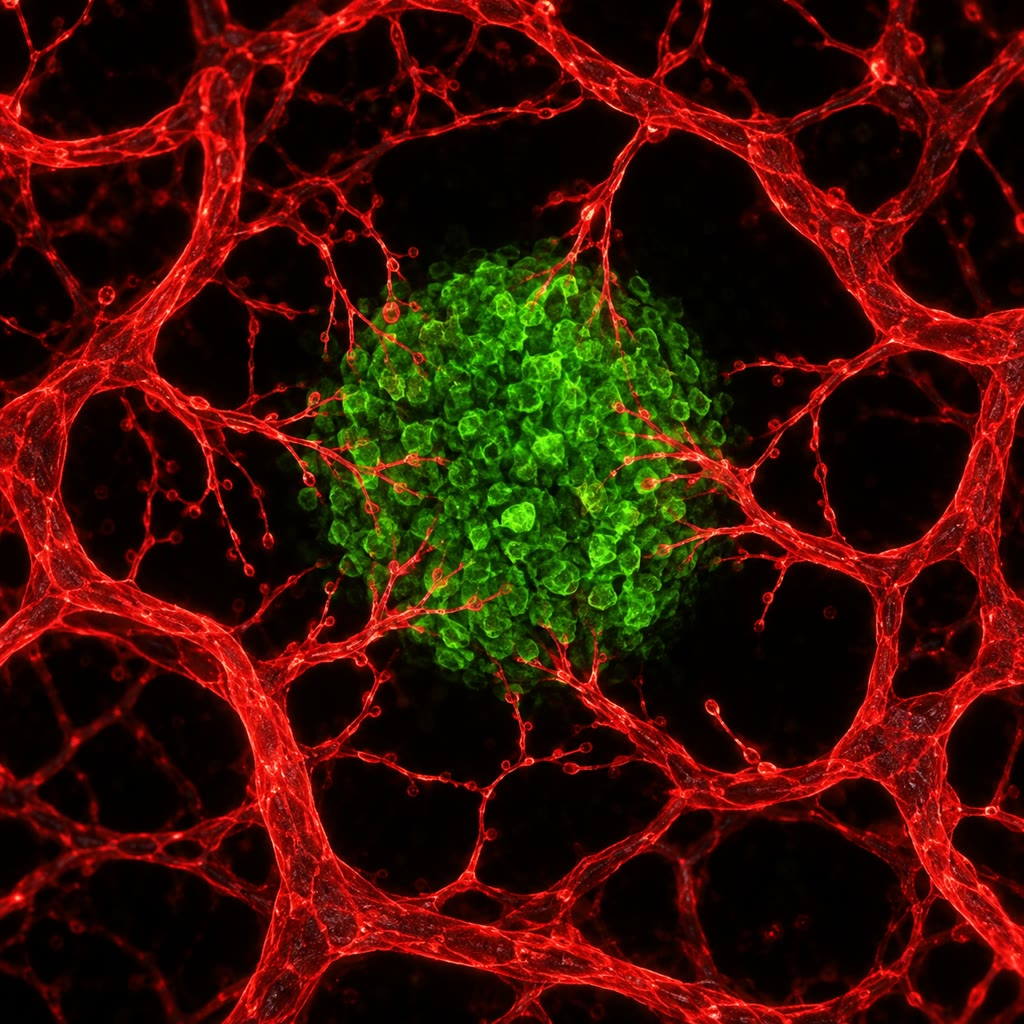
\includegraphics[width=0.36\linewidth]{images/book5/ai/b5-11-angiogenesis.jpg}\hspace{0.04\linewidth}
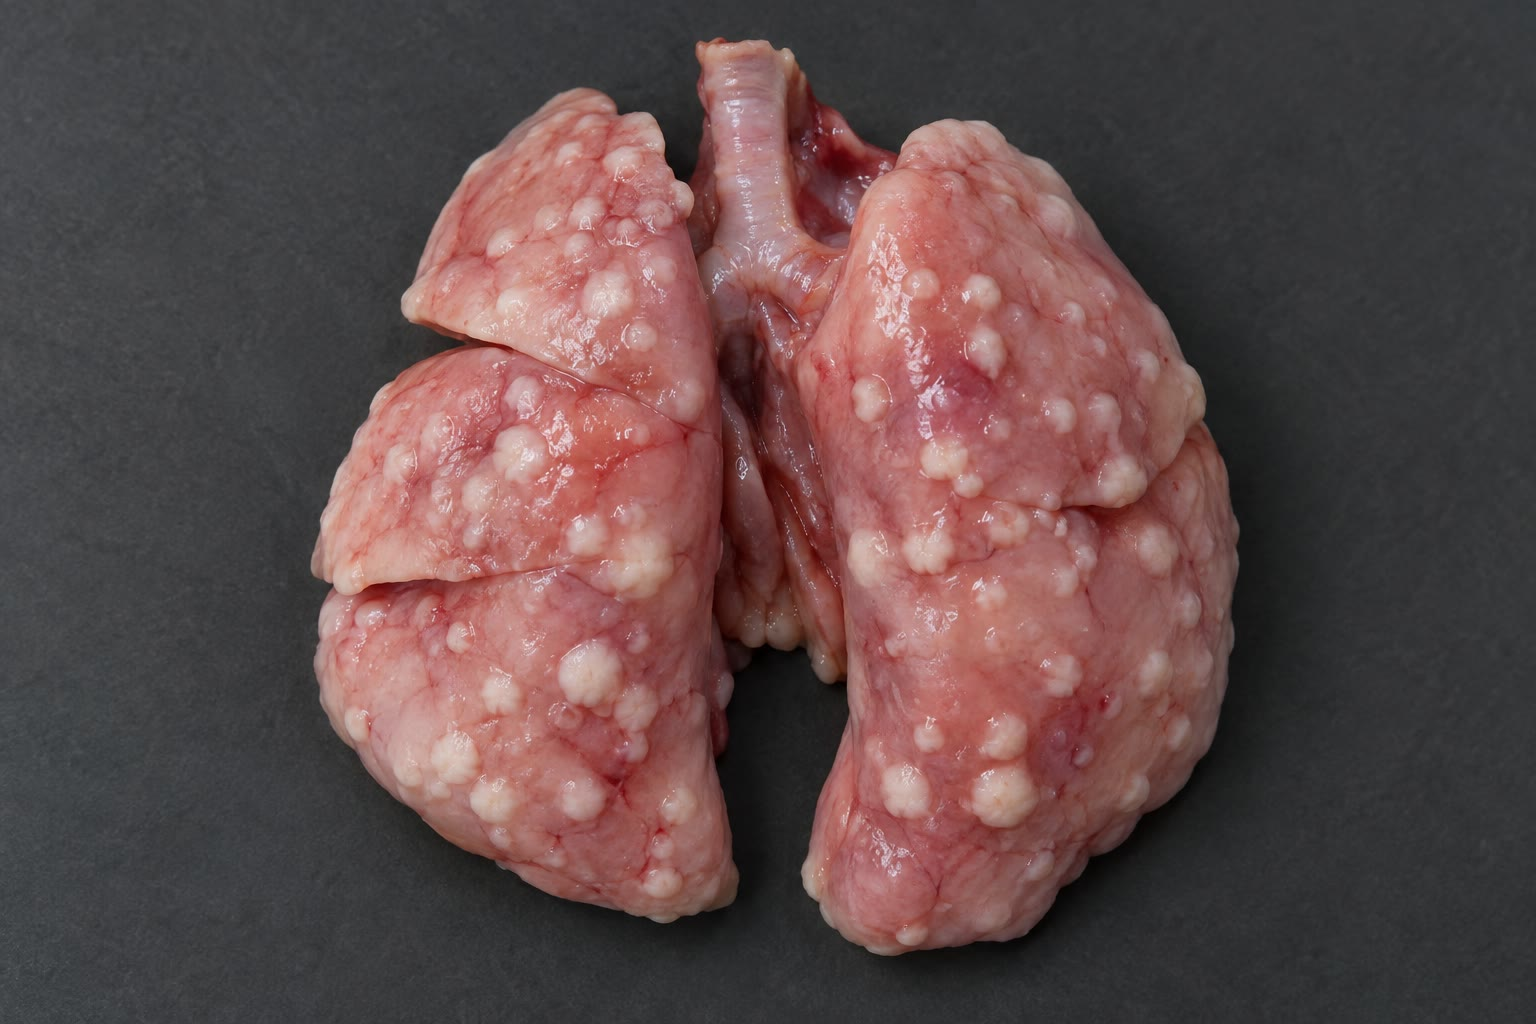
\includegraphics[width=0.54\linewidth]{images/book5/ai/b5-11-metastasis-lung.jpg}

{\small À gauche~: un sphéroïde tumoral (vert) qui recrute de nouveaux
vaisseaux (rouge) dans un réseau voisin --- l'angiogenèse en culture. À
droite~: un poumon de souris criblé de \omterm{def:b3:cancer-biology:hallmarks}{métastases}, chaque colonie
fondée par une cellule qui a survécu au voyage dans le sang.}
\end{omfigure}

\begin{definition}[Invasion et métastase]\label{def:b3:cancer-biology:metastasis}
\index{invasion}\index{transition épithélio-mésenchymateuse}\index{la graine et le terrain}
Pour métastaser, une cellule de carcinome doit quitter l'épithélium ---
perdre ses jonctions et sa polarité et acquérir la motilité, une
\emph{transition épithélio-mésenchymateuse} commandée par des facteurs
de transcription qui servent normalement au développement embryonnaire
--- dégrader la lame basale et la matrice par des protéases sécrétées,
franchir la paroi d'un vaisseau sanguin ou lymphatique, survivre dans
la circulation (moins d'une sur dix mille y parvient, tuées par le
cisaillement, par l'absence d'ancrage et par les cellules tueuses
naturelles), se loger dans un lit capillaire d'un autre organe, en
sortir et y croître. L'endroit où elle croît n'est pas aléatoire~: le
\omterm{def:b3:cancer-biology:hallmarks}{cancer} du sein va à l'os, au poumon, au foie et au cerveau, celui du
côlon au foie, celui de la prostate à l'os --- \emph{la graine et le
terrain} de Paget (1889), qu'expliquent en partie le débit sanguin et
en partie l'accord entre la cellule et les signaux du tissu. Une
cellule disséminée peut rester dormante des années avant de croître, ce
qui explique que des \omterm{def:b3:cancer-biology:hallmarks}{cancers} récidivent dix ans après une guérison
apparente. La \omterm{def:b3:cancer-biology:hallmarks}{métastase} cause neuf morts sur dix par \omterm{def:b3:cancer-biology:hallmarks}{tumeur} solide, et
c'est l'étape la moins comprise.
\end{definition}

\begin{proposition}[Échapper au système immunitaire]\label{prop:b3:cancer-biology:immune}
\index{échappement immunitaire}\index{inhibiteur de point de contrôle}\index{néoantigène}
Les mutations d'une \omterm{def:b3:cancer-biology:hallmarks}{tumeur} créent des \emph{néoantigènes}, peptides
qu'aucune cellule normale ne présente, et les lymphocytes~T
cytotoxiques reconnaissent et tuent les cellules tumorales --- d'où le
fait que les patients immunodéprimés font plus de \omterm{def:b3:cancer-biology:hallmarks}{cancers} et que les
\omterm{def:b3:cancer-biology:hallmarks}{tumeurs} très mutées (mélanome, poumon, côlon déficient en \omterm{prop:b3:dna-repair:fidelity}{réparation
des mésappariements}) répondent le mieux à l'immunothérapie. Une \omterm{def:b3:cancer-biology:hallmarks}{tumeur}
cliniquement visible est une \omterm{def:b3:cancer-biology:hallmarks}{tumeur} qui a échappé~: en perdant les
molécules du CMH qui présentent les peptides, en sécrétant des facteurs
suppresseurs, en recrutant des lymphocytes~T régulateurs et, surtout,
en exprimant PD-L1, qui engage le récepteur inhibiteur PD-1 des
lymphocytes~T et les éteint, le frein même qui met normalement fin à
une réponse immunitaire (\cref{ch:b3:adaptive-immunity}). Les anticorps
qui bloquent PD-1 ou PD-L1, ou le frein plus précoce CTLA-4, libèrent
les lymphocytes~T~; chez une fraction des patients --- d'un cinquième à
la moitié selon la \omterm{def:b3:cancer-biology:hallmarks}{tumeur} --- ils produisent des rémissions durables de
\omterm{def:b3:cancer-biology:hallmarks}{cancers} jusque-là incurables, et leurs effets indésirables sont des
auto-immunités, l'autre fonction du frein.
\end{proposition}

\section{Causes et traitements}

\begin{proposition}[Les causes]\label{prop:b3:cancer-biology:causes}
\index{cancérogène}\index{virus oncogène}
Le \omterm{def:b3:cancer-biology:hallmarks}{cancer} est causé par tout ce qui augmente la vitesse des événements
du théorème ou le nombre de cellules exposées. Les \emph{cancérogènes
chimiques}, mutagènes pour la plupart après activation par le foie~:
les soixante-dix cancérogènes de la fumée de tabac, qui causent un
tiers des morts par \omterm{def:b3:cancer-biology:hallmarks}{cancer} et multiplient par quinze à vingt-cinq le
risque de \omterm{def:b3:cancer-biology:hallmarks}{cancer} du poumon~; l'aflatoxine des grains moisis~;
l'amiante, qui n'est pas un mutagène mais un irritant chronique. Les
\emph{rayonnements}~: l'ultraviolet pour la peau (les dimères du
\cref{ch:b3:dna-repair}), les rayonnements ionisants pour les leucémies,
la thyroïde et le sein. Les \emph{infections}, un sixième des \omterm{def:b3:cancer-biology:hallmarks}{cancers}
dans le monde~: les papillomavirus, dont les protéines E6 et E7
détruisent \omterm{def:b3:cancer-biology:genes}{p53} et inactivent Rb et causent presque tous les \omterm{def:b3:cancer-biology:hallmarks}{cancers} du
col de l'utérus (un vaccin les prévient désormais)~; les virus des
hépatites B et C dans le \omterm{def:b3:cancer-biology:hallmarks}{cancer} du foie~; le virus d'Epstein--Barr dans
des lymphomes~; \emph{Helicobacter pylori} dans le \omterm{def:b3:cancer-biology:hallmarks}{cancer} de l'estomac,
par des décennies d'inflammation. Les \emph{mutations héritées} d'un
suppresseur de \omterm{def:b3:cancer-biology:hallmarks}{tumeur}, premier coup dès la naissance, dans quelque
\qty{5}{\%} des \omterm{def:b3:cancer-biology:hallmarks}{cancers}. Et le hasard~: la plupart des mutations d'une
\omterm{def:b3:cancer-biology:hallmarks}{tumeur} viennent des erreurs ordinaires de la réplication, de sorte que
les tissus qui se divisent le plus --- côlon, peau, sang --- ont le
plus de \omterm{def:b3:cancer-biology:hallmarks}{cancers}, et que le risque croît avec l'âge quoi qu'on fasse.
\end{proposition}

\begin{theorem}[Pourquoi un médicament échoue et deux peut-être pas]\label{thm:b3:cancer-biology:goldie-coldman}
\index{modèle de Goldie--Coldman}\index{résistance aux médicaments}\index{polythérapie}
Soit une \omterm{def:b3:cancer-biology:hallmarks}{tumeur} de $N$ cellules produite par divisions successives à
partir d'une cellule, et soit $\mu$ la vitesse à laquelle apparaît, par
division cellulaire, une mutation conférant la résistance à un
médicament donné. La probabilité que la \omterm{def:b3:cancer-biology:hallmarks}{tumeur} ne contienne
\emph{aucune} cellule résistante au début du traitement vaut alors à peu
près
\[
P_{0} \approx e^{-\mu N},
\]
de sorte que pour $\mu N \gg 1$ la résistance préexiste presque à coup
sûr. Pour deux médicaments à mécanismes de résistance indépendants, une
cellule résistante aux deux apparaît à la vitesse d'environ
$\mu_{1}\mu_{2}$ par division, et $P_{0}
\approx e^{-\mu_{1}\mu_{2}N}$~: avec $N = 10^{9}$ et $\mu = 10^{-7}$, un
seul médicament affronte en moyenne $\mu N = 100$ clones résistants,
deux médicaments une probabilité de $10^{-5}$ qu'il existe ne
serait-ce qu'une cellule doublement résistante.
\end{theorem}
\begin{proof}[Démonstration partielle]
Croître de $1$ à $N$ cellules demande environ $N$ divisions en tout (un
arbre à $N$ feuilles a $N - 1$ nœuds internes). Si une cellule
résistante est produite à chaque division avec la probabilité $\mu$ et
que, en première approximation, sa descendance ne meurt ni ne dépasse
le reste, le nombre d'événements de résistance suit une loi de Poisson
de moyenne $\mu N$, et la probabilité qu'il n'y en ait aucun vaut
$e^{-\mu N}$. Des mécanismes indépendants multiplient les probabilités
par division. L'approximation néglige le fait que les mutants précoces
laissent des clones résistants plus grands --- la distribution complète
est celle de Luria et Delbrück, traitée dans le volume de deuxième
année --- mais la probabilité qu'il n'y ait \emph{aucun} mutant, qui
décide si la \omterm{def:b3:cancer-biology:hallmarks}{tumeur} peut être guérie, est exactement le terme de
Poisson.
\end{proof}

\begin{example}[Les traitements et leur logique]\label{ex:b3:cancer-biology:therapy}
La chirurgie et la radiothérapie retirent ou tuent une \omterm{def:b3:cancer-biology:hallmarks}{tumeur}
localisée~; le rayonnement tue par \omterm{def:b3:dna-repair:lesions}{cassures double brin}, et son
fractionnement en doses quotidiennes laisse le tissu sain réparer entre
elles (\cref{ch:b3:dna-repair}). La chimiothérapie cytotoxique ---
agents alkylants, antimétabolites, poisons des \omterm{def:b3:cytoskeleton-motility:filaments}{microtubules},
inhibiteurs des topo-isomérases --- tue les cellules en division de
toute sorte, les cellules tumorales un peu plus, et obéit à une
\emph{loi de destruction logarithmique}~: chaque cure tue une fraction
constante, disons \qty{99}{\%}, de sorte que six cures ramènent
$10^{12}$ cellules à une, et qu'il faut les mêmes six cures que la
\omterm{def:b3:cancer-biology:hallmarks}{tumeur} soit grande ou petite~; les cheveux, l'intestin et la moelle du
patient, qui se divisent aussi, fixent la dose. La thérapie ciblée
s'attaque à une lésion dont la \omterm{def:b3:cancer-biology:hallmarks}{tumeur} dépend~: l'imatinib bloque la
kinase BCR--ABL et a fait de la leucémie myéloïde chronique une maladie
chronique au lieu d'une maladie mortelle~; le trastuzumab se fixe sur
HER2~; les inhibiteurs de PARP, les inhibiteurs de Cdk4/6 et le
vénétoclax des chapitres précédents exploitent chacun un défaut.
L'immunothérapie libère les lymphocytes~T. Et le théorème dit comment
les employer~: en association, tôt, quand $N$ est le plus petit ---
c'est ce que fait la chimiothérapie adjuvante après une chirurgie ---
et avec des médicaments dont les mécanismes de résistance ne se
recouvrent pas. La \omterm{def:b3:cancer-biology:hallmarks}{tumeur} est une population qui évolue, et le
traitement est une sélection.
\end{example}

\begin{omfigure}
\begin{tikzpicture}
\begin{axis}[
  width=0.7\linewidth, height=5.6cm,
  axis x line=bottom, axis y line=left,
  xmin=0, xmax=8, ymin=1, ymax=1e13, ymode=log,
  xlabel={cures de chimiothérapie}, ylabel={cellules tumorales},
  xlabel style={font=\small, at={(axis description cs:0.5,-0.12)}, anchor=north},
  ylabel style={font=\small},
  tick label style={font=\small}, xtick={0,2,4,6,8},
  clip=false,
]
\addplot[very thick, omDef, mark=*, mark size=1.2pt] coordinates {(0,1e12) (1,1e10) (2,1e8) (3,1e6) (4,1e4) (5,1e2) (6,1)};
\addplot[very thick, omThm, mark=*, mark size=1.2pt] coordinates {(0,1e12) (1,1.01e10) (2,1.02e8) (3,1.04e6) (4,1.1e4) (5,200) (6,300) (7,600) (8,1200)};
\addplot[dashed, gray, domain=0:8, samples=2] {1e9};
\node[font=\scriptsize, gray, anchor=south west] at (axis cs:0.2,1.3e9) {détectable, $10^{9}$};
\node[font=\scriptsize, omDef, anchor=south west] at (axis cs:0.3,1e4) {\qty{99}{\%} tués par cure};
\node[font=\scriptsize, omThm, anchor=south west] at (axis cs:5.2,3e3) {une cellule résistante au départ~: rechute};
\end{axis}
\end{tikzpicture}

{\small La loi de destruction logarithmique. Chaque cure tue la même
fraction des cellules, de sorte que la \omterm{def:b3:cancer-biology:hallmarks}{tumeur} perd un nombre fixe de
décades par cure et devient indétectable bien avant d'avoir disparu
(bleu)~; une unique cellule résistante préexistante survit à chaque
cure et repeuple (rouge).}
\end{omfigure}

\begin{remark}[Ce qui a changé]\label{rem:b3:cancer-biology:changed}
La moitié des patients chez qui l'on diagnostique un \omterm{def:b3:cancer-biology:hallmarks}{cancer} dans un
pays riche survivent aujourd'hui dix ans, contre un quart en 1970. Le
gain est venu de la prévention (tabac, vaccins contre l'hépatite et le
papillomavirus, dépistage des polypes et des lésions du col), d'une
détection plus précoce, et de traitements qui découlent de la biologie
de ce chapitre --- la polychimiothérapie qui guérit la plupart des
leucémies de l'enfant et des \omterm{def:b3:cancer-biology:hallmarks}{cancers} du testicule, les médicaments
ciblés et les immunothérapies. Ce qui n'a pas changé est la maladie
métastatique, que la biologie explique mais ne guérit pas encore~; les
gains suivants viendront de ce qu'on traitera la \omterm{def:b3:cancer-biology:hallmarks}{tumeur} pour ce qu'elle
est, une population qui évolue sous la sélection qu'impose le
traitement.
\end{remark}

\section{Exercices}

\begin{exercise}[$\star$]\label{exo:b3:cancer-biology:1}
Distinguer un \omterm{def:b3:cancer-biology:genes}{oncogène} d'un \omterm{def:b3:cancer-biology:genes}{gène suppresseur de tumeur} par le
mécanisme, par le nombre d'allèles qui doivent changer, et par deux
exemples de chaque.
\end{exercise}

\begin{exercise}[$\star$]\label{exo:b3:cancer-biology:2}
Énumérer les \omterm{def:b3:cancer-biology:hallmarks}{caractères distinctifs du cancer} et, pour chacun, nommer
un gène de ce chapitre ou d'un chapitre précédent dont l'altération le
procure.
\end{exercise}

\begin{exercise}[$\star$]\label{exo:b3:cancer-biology:3}
Qu'a observé Knudson à propos du rétinoblastome héréditaire et du
rétinoblastome sporadique, et qu'en a-t-il inféré~?
\end{exercise}

\begin{exercise}[$\star$]\label{exo:b3:cancer-biology:4}
Expliquer le \omterm{met:b3:cancer-biology:ames}{test d'Ames} et pourquoi on y ajoute un extrait de foie.
\end{exercise}

\begin{exercise}[$\star\star$]\label{exo:b3:cancer-biology:5}
L'incidence d'un \omterm{def:b3:cancer-biology:hallmarks}{cancer} vaut $2\times 10^{-5}$ par an à $40$ ans et
$2\times 10^{-3}$ à $80$ ans. Estimer l'exposant de la loi de puissance
en l'âge et le nombre d'événements limitants qu'il suggère.
\end{exercise}

\begin{exercise}[$\star\star$]\label{exo:b3:cancer-biology:6}
À l'aide de la \cref{prop:b3:cancer-biology:oxygen} avec $D =
\qty{2e-9}{m^2/s}$ et $c_{0} = \qty{0.05}{mol/m^3}$, calculer $L$ pour
un tissu qui consomme \qty{0.01}{mol/m^3/s} et pour une \omterm{def:b3:cancer-biology:hallmarks}{tumeur} qui en
consomme trois fois plus. Pourquoi une \omterm{def:b3:cancer-biology:hallmarks}{tumeur} à croissance rapide
devient-elle nécrotique plus tôt~?
\end{exercise}

\begin{exercise}[$\star\star$]\label{exo:b3:cancer-biology:7}
Une \omterm{def:b3:cancer-biology:hallmarks}{tumeur} de $10^{11}$ cellules est traitée par un médicament qui en
tue \qty{99.9}{\%} par cure. Combien de cures pour la réduire au-dessous
d'une cellule~? Pourquoi la \omterm{def:b3:cancer-biology:hallmarks}{tumeur} est-elle indétectable après deux
cures alors qu'il reste $10^{5}$ cellules, et qu'est-ce que cela
implique pour l'arrêt du traitement~?
\end{exercise}

\begin{exercise}[$\star\star$]\label{exo:b3:cancer-biology:8}
Expliquer pourquoi une mutation d'EGFR et une mutation de KRAS se
trouvent rarement dans une même \omterm{def:b3:cancer-biology:hallmarks}{tumeur} du poumon, et pourquoi une
\omterm{def:b3:cancer-biology:hallmarks}{tumeur} traitée par un inhibiteur d'EGFR rechute souvent avec une
mutation de KRAS.
\end{exercise}

\begin{exercise}[$\star\star$]\label{exo:b3:cancer-biology:9}
Les protéines E6 et E7 du papillomavirus inactivent \omterm{def:b3:cancer-biology:genes}{p53} et Rb.
Expliquer comment cela entraîne un \omterm{def:b3:cancer-biology:hallmarks}{cancer} du col de l'utérus, pourquoi
cela prend des décennies, et pourquoi un vaccin administré avant le
début de la vie sexuelle le prévient.
\end{exercise}

\begin{exercise}[$\star\star\star$]\label{exo:b3:cancer-biology:10}
Étendre l'argument d'Armitage--Doll pour permettre à chaque coup de
faire croître son clone d'un facteur $g$ avant le suivant~: montrer que
l'incidence garde la même puissance de $t$ mais un préfacteur multiplié
par $g^{k-1}$, et discuter pourquoi le $k$ ajusté sur une courbe d'âge
est un majorant du nombre de \omterm{prop:b3:cancer-biology:multistep}{mutations motrices}.
\end{exercise}

\begin{exercise}[$\star\star\star$]\label{exo:b3:cancer-biology:11}
À l'aide du \cref{thm:b3:cancer-biology:goldie-coldman}, comparer
(a) traiter une \omterm{def:b3:cancer-biology:hallmarks}{tumeur} de $10^{9}$ cellules par le médicament A pendant
six cures puis par le médicament B pendant six, et (b) donner A et B
ensemble dès le début, lorsque $\mu_{A} =
\mu_{B} = 10^{-7}$. Calculer $P_{0}$ pour chaque stratégie et expliquer
pourquoi l'association précoce est la règle.
\end{exercise}

\begin{exercise}[$\star\star\star$]\label{exo:b3:cancer-biology:12}
Le paradoxe de Peto~: un éléphant a cent fois plus de cellules qu'un
homme et vit aussi longtemps, et pourtant il n'a pas plus de \omterm{def:b3:cancer-biology:hallmarks}{cancers}. À
l'aide du théorème de ce chapitre, dire quelle est l'attente naïve, et
proposer deux mécanismes par lesquels les grands animaux auraient pu
résoudre le problème (l'éléphant a vingt copies de \emph{TP53}).
\end{exercise}

\section{Problème~: l'arithmétique d'une tumeur}

\begin{problem}[{Problème du week-end --- une tumeur poussée à partir
d'une cellule et chronométrée jusqu'à sa détection, sa courbe d'âge lue
pour en tirer le nombre de coups, son alimentation en dioxygène et son
cœur nécrotique calculés, et son traitement planifié contre la
certitude de la résistance, pour finir sur les années jusqu'à la
détection, l'épaisseur de tumeur vivante autour d'un vaisseau et la
probabilité qu'une association guérisse}]
\label{pb:b3:cancer-biology:1}
Données~: une cellule tumorale a un volume de \qty{1000}{\micro m^3}~;
temps de doublement \qty{100}{d}~; détection à \qty{1}{cm^3}~; charge
létale \qty{1}{kg}. Courbe d'âge~: incidence $1\times 10^{-5}$ par an à
$30$ ans et $3\times
10^{-3}$ à $80$ ans. Dioxygène~: $D = \qty{2e-9}{m^2/s}$, $c_{0} =
\qty{0.05}{mol/m^3}$, $q = \qty{0.03}{mol/m^3/s}$ dans la \omterm{def:b3:cancer-biology:hallmarks}{tumeur}~; dans
une \omterm{def:b3:cancer-biology:hallmarks}{tumeur} vascularisée les capillaires sont distants de
\qty{150}{\micro m}. Traitement~: chaque cure tue \qty{99}{\%}~; taux de
mutation de résistance $10^{-7}$ par division et par médicament~; une
cure toutes les trois semaines~; la \omterm{def:b3:cancer-biology:hallmarks}{tumeur} repousse entre les cures
avec le même temps de doublement.

\medskip
\noindent\textbf{Partie I --- La croissance.}
\begin{enumerate}
  \item Combien de cellules dans \qty{1}{cm^3}~? Combien de doublements
        depuis une cellule~?
  \item Combien d'années de la cellule fondatrice à la détection~?
  \item Combien de doublements, et d'années, de la détection à la
        charge létale~? Comparer les deux intervalles.
  \item Beaucoup de \omterm{def:b3:cancer-biology:hallmarks}{tumeurs} sont détectées à \qty{1}{cm^3} mais ne
        croissaient que depuis cinq ans. Qu'a-t-il fallu qu'il en soit
        du temps de doublement au début, ou de la loi de croissance~?
  \item Une fraction $f$ seulement des cellules d'une \omterm{def:b3:cancer-biology:hallmarks}{tumeur} se divise
        à un instant donné (la fraction de croissance), et une fraction
        meurt. Si les cellules cyclent en \qty{2}{d} mais que la \omterm{def:b3:cancer-biology:hallmarks}{tumeur}
        double en $100$, que dit cela de l'équilibre entre naissances
        et morts~?
  \item Pourquoi la même chimiothérapie à destruction logarithmique
        épargne-t-elle davantage une \omterm{def:b3:cancer-biology:hallmarks}{tumeur} à croissance lente qu'une
        \omterm{def:b3:cancer-biology:hallmarks}{tumeur} rapide, et pourquoi la rapide repousse-t-elle malgré
        tout plus vite entre les cures~?
\end{enumerate}

\medskip
\noindent\textbf{Partie II --- Les coups.}
\begin{enumerate}[resume]
  \item À partir des deux incidences, calculer l'exposant $k - 1$ de la
        courbe d'âge et le nombre d'événements $k$ qu'il implique.
  \item Si chaque événement survient à $u = 10^{-6}$ par cellule et par
        an dans $N = 10^{8}$ cellules sensibles, que prédit le théorème
        pour le risque cumulé à $70$ ans avec votre $k$~? Est-ce
        plausible~? Que manque-t-il~?
  \item Recommencer avec une expansion clonale d'un facteur $g = 100$
        après chacun des $k - 1$ premiers coups, en s'aidant de
        l'\cref{exo:b3:cancer-biology:10}.
  \item Une porteuse hérite d'un coup. De quel facteur son incidence à
        $40$ ans est-elle augmentée, si les autres vitesses sont
        inchangées~? (Comparer $(ut)^{k-1}$ et $(ut)^{k}$ en
        $t = 40$.)
  \item Le tabac multiplie le $u$ de l'un des événements par $10$. De
        quel facteur l'incidence monte-t-elle si cet événement est l'un
        des $k$~; s'il en concerne deux~?
  \item Expliquer pourquoi arrêter de fumer à cinquante ans abaisse le
        risque de \omterm{def:b3:cancer-biology:hallmarks}{cancer} du poumon au-dessous de celui d'un fumeur qui
        continue, mais jamais jusqu'à celui d'une personne n'ayant
        jamais fumé.
\end{enumerate}

\medskip
\noindent\textbf{Partie III --- L'alimentation.}
\begin{enumerate}[resume]
  \item Calculer la profondeur de pénétration du dioxygène $L$ dans la
        \omterm{def:b3:cancer-biology:hallmarks}{tumeur}.
  \item Un sphéroïde sans vaisseaux~: quel est le diamètre maximal pour
        lequel chaque cellule est oxygénée~? Quelle est l'épaisseur du
        pourtour vivant d'un sphéroïde de \qty{2}{mm}, et quelle
        fraction de son volume est vivante~?
  \item Dans une \omterm{def:b3:cancer-biology:hallmarks}{tumeur} vascularisée dont les capillaires sont distants
        de \qty{150}{\micro m}, chaque cellule est-elle oxygénée~?
        Quelles cellules sont hypoxiques, et pourquoi cela compte-t-il
        pour la radiothérapie (le dioxygène fixe les dégâts du
        rayonnement) et pour la sélection des cellules à \omterm{def:b3:cancer-biology:genes}{p53} mutée~?
  \item Un médicament divise par deux la densité capillaire de la
        \omterm{def:b3:cancer-biology:hallmarks}{tumeur}. Recalculer l'espacement et dire ce qu'il advient des
        cellules à mi-distance entre vaisseaux.
  \item Les cellules hypoxiques passent à la glycolyse, qui fait
        \qty{2}{ATP} par glucose au lieu de $30$. De quel facteur
        doivent-elles augmenter leur capture de glucose pour maintenir
        leur ATP, et comment l'exploite-t-on en imagerie des \omterm{def:b3:cancer-biology:hallmarks}{tumeurs}~?
  \item Expliquer pourquoi un traitement anti-angiogénique seul guérit
        rarement mais peut aider la chimiothérapie à atteindre la
        \omterm{def:b3:cancer-biology:hallmarks}{tumeur}.
\end{enumerate}

\medskip
\noindent\textbf{Partie IV --- Le traitement.}
\begin{enumerate}[resume]
  \item Une \omterm{def:b3:cancer-biology:hallmarks}{tumeur} de \qty{1}{cm^3} est traitée par un seul médicament.
        Combien de cures la réduisent au-dessous d'une cellule, en
        négligeant la repousse et la résistance~?
  \item Entre les cures (trois semaines) les survivantes repoussent. De
        quel facteur~? Recalculer la destruction nette par cycle et le
        nombre de cycles nécessaires.
  \item Calculer le nombre espéré de cellules résistantes au médicament
        au début du traitement et la probabilité qu'il n'y en ait
        aucune.
  \item Deux médicaments à mécanismes indépendants sont donnés
        ensemble. Probabilité qu'aucune cellule doublement résistante
        n'existe au début~? Et pour une \omterm{def:b3:cancer-biology:hallmarks}{tumeur} de $10^{12}$ cellules~?
  \item Le traitement adjuvant est donné après une chirurgie, quand il
        reste peut-être $10^{6}$ cellules non détectées. Recalculer les
        probabilités pour un et pour deux médicaments, et énoncer la
        leçon.
  \item Une immunothérapie suscite des lymphocytes~T qui tuent toute
        cellule présentant un néoantigène. Pourquoi la résistance à
        cette thérapie est-elle un problème différent de la résistance
        à un inhibiteur de kinase, et sur quelles \omterm{def:b3:cancer-biology:hallmarks}{tumeurs} le théorème
        suggère-t-il qu'elle marche le mieux~?
  \item Résumer~: les années de la cellule fondatrice à la détection
        (question~2), l'épaisseur de \omterm{def:b3:cancer-biology:hallmarks}{tumeur} vivante autour d'un
        vaisseau (question~13) et la probabilité que l'association de
        deux médicaments n'affronte aucune cellule résistante dans une
        \omterm{def:b3:cancer-biology:hallmarks}{tumeur} de \qty{1}{cm^3} (question~22).
\end{enumerate}
\end{problem}
